\begin{center}
	\LARGE Uden hjælpemidler
\end{center}
\begin{opgavetekst}{Opgave 1}
\end{opgavetekst}
\begin{delopgave}{}{1}
	Udregn følgende logaritmer.
	\begin{align*}
		&1) \ \ln(e^3) &   &2) \log_{10}(1000)\\
		&3) \ \log_2(32) &   & 4) \log_5(125) 
	\end{align*}
\end{delopgave}
%%%%%%%%%%%%%%%%%%%%%%%%%%%%%%%%%%%%%%%%%%%%%%%%%%%%%%%%%%%%%%%%%%%%%%%%%%%%%%%%%%%%%%%%%%%%%%%%
%%%%%%%%%%%%%%%%%%%%%%%%%%%%%%%%%%%%%%%%%%%%%%%%%%%%%%%%%%%%%%%%%%%%%%%%%%%%%%%%%%%%%%%%%%%%%%%%
%%%%%%%%%%%%%%%%%%%%%%%%%%%%%%%%%%%%%%%%%%%%%%%%%%%%%%%%%%%%%%%%%%%%%%%%%%%%%%%%%%%%%%%%%%%%%%%%
%%%%%%%%%%%%%%%%%%%%%%%%%%%%%%%%%%%%%%%%%%%%%%%%%%%%%%%%%%%%%%%%%%%%%%%%%%%%%%%%%%%%%%%%%%%%%%%%
%%%%%%%%%%%%%%%%%%%%%%%%%%%%%%%%%%%%%%%%%%%%%%%%%%%%%%%%%%%%%%%%%%%%%%%%%%%%%%%%%%%%%%%%%%%%%%%%
%%%%%%%%%%%%%%%%%%%%%%%%%%%%%%%%%%%%%%%%%%%%%%%%%%%%%%%%%%%%%%%%%%%%%%%%%%%%%%%%%%%%%%%%%%%%%%%%
%%%%%%%%%%%%%%%%%%%%%%%%%%%%%%%%%%%%%%%%%%%%%%%%%%%%%%%%%%%%%%%%%%%%%%%%%%%%%%%%%%%%%%%%%%%%%%%%
%%%%%%%%%%%%%%%%%%%%%%%%%%%%%%%%%%%%%%%%%%%%%%%%%%%%%%%%%%%%%%%%%%%%%%%%%%%%%%%%%%%%%%%%%%%%%%%%
\begin{opgavetekst}{Opgave 2}
	Grafen for en funktion $f$ går gennem punkterne $(1,8)$ og $(4,64)$. Forskriften for $f$ er givet ved
	\begin{align*}
		f(x) = b\cdot a^x.
	\end{align*}
\end{opgavetekst}
\begin{delopgave}{}{1}
	Brug punkterne til at bestemme tallene $b$ og $a$.
\end{delopgave}
\begin{delopgave}{}{2}
	Bestem $f(3)$.
\end{delopgave}
%%%%%%%%%%%%%%%%%%%%%%%%%%%%%%%%%%%%%%%%%%%%%%%%%%%%%%%%%%%%%%%%%%%%%%%%%%%%%%%%%%%%%%%%%%%%%%%%
%%%%%%%%%%%%%%%%%%%%%%%%%%%%%%%%%%%%%%%%%%%%%%%%%%%%%%%%%%%%%%%%%%%%%%%%%%%%%%%%%%%%%%%%%%%%%%%%
%%%%%%%%%%%%%%%%%%%%%%%%%%%%%%%%%%%%%%%%%%%%%%%%%%%%%%%%%%%%%%%%%%%%%%%%%%%%%%%%%%%%%%%%%%%%%%%%
%%%%%%%%%%%%%%%%%%%%%%%%%%%%%%%%%%%%%%%%%%%%%%%%%%%%%%%%%%%%%%%%%%%%%%%%%%%%%%%%%%%%%%%%%%%%%%%%
%%%%%%%%%%%%%%%%%%%%%%%%%%%%%%%%%%%%%%%%%%%%%%%%%%%%%%%%%%%%%%%%%%%%%%%%%%%%%%%%%%%%%%%%%%%%%%%%
%%%%%%%%%%%%%%%%%%%%%%%%%%%%%%%%%%%%%%%%%%%%%%%%%%%%%%%%%%%%%%%%%%%%%%%%%%%%%%%%%%%%%%%%%%%%%%%%
%%%%%%%%%%%%%%%%%%%%%%%%%%%%%%%%%%%%%%%%%%%%%%%%%%%%%%%%%%%%%%%%%%%%%%%%%%%%%%%%%%%%%%%%%%%%%%%%
%%%%%%%%%%%%%%%%%%%%%%%%%%%%%%%%%%%%%%%%%%%%%%%%%%%%%%%%%%%%%%%%%%%%%%%%%%%%%%%%%%%%%%%%%%%%%%%%
\newpage
\begin{opgavetekst}{Opgave 3}
	På Figur \ref{fig:potensgraf} ses grafen for en potensfunktion $f$.
	\begin{figure}[H]
		\centering
		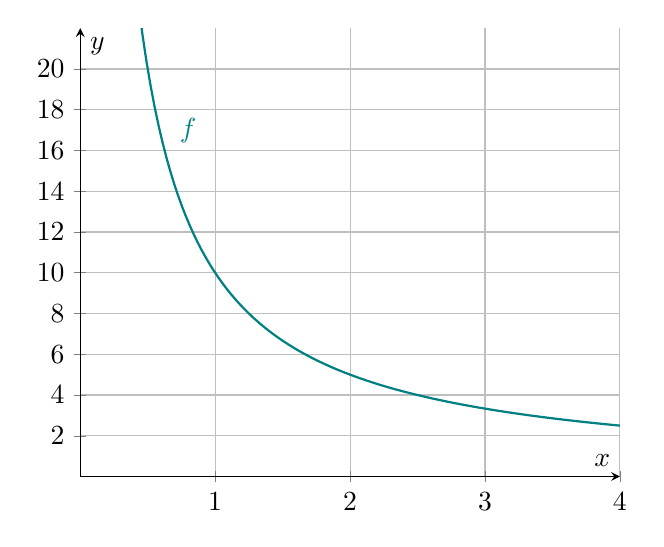
\begin{tikzpicture}
			\begin{axis}[
				axis lines = middle, 
				xmin = 0, xmax = 4, 
				ymin = 0, ymax = 22,
				grid = both, 
				ytick = {0,2,...,20},
				xlabel = $x$, ylabel = $y$
				]
				\addplot[thick, color = teal, domain = 0.2:6, samples = 200] {10*x^(-1)};
				\node[color = teal] at (axis cs: 0.8,17) {$f$};
			\end{axis}
		\end{tikzpicture}
		\caption{Graf for potensfunktionen $f$}
		\label{fig:potensgraf}
	\end{figure}
	\phantom{h}
\end{opgavetekst}
\begin{delopgave}{}{1}
	Bestem $b$-værdien for $f$.
\end{delopgave}
\begin{delopgave}{}{2}
	Bestem $f(0.5)$.
\end{delopgave}
\begin{delopgave}{}{3}
	Løs ligningen $f(x) = 4$.
\end{delopgave}
%%%%%%%%%%%%%%%%%%%%%%%%%%%%%%%%%%%%%%%%%%%%%%%%%%%%%%%%%%%%%%%%%%%%%%%%%%%%%%%%%%%%%%%%%%%%%%%%
%%%%%%%%%%%%%%%%%%%%%%%%%%%%%%%%%%%%%%%%%%%%%%%%%%%%%%%%%%%%%%%%%%%%%%%%%%%%%%%%%%%%%%%%%%%%%%%%
%%%%%%%%%%%%%%%%%%%%%%%%%%%%%%%%%%%%%%%%%%%%%%%%%%%%%%%%%%%%%%%%%%%%%%%%%%%%%%%%%%%%%%%%%%%%%%%%
%%%%%%%%%%%%%%%%%%%%%%%%%%%%%%%%%%%%%%%%%%%%%%%%%%%%%%%%%%%%%%%%%%%%%%%%%%%%%%%%%%%%%%%%%%%%%%%%
%%%%%%%%%%%%%%%%%%%%%%%%%%%%%%%%%%%%%%%%%%%%%%%%%%%%%%%%%%%%%%%%%%%%%%%%%%%%%%%%%%%%%%%%%%%%%%%%
%%%%%%%%%%%%%%%%%%%%%%%%%%%%%%%%%%%%%%%%%%%%%%%%%%%%%%%%%%%%%%%%%%%%%%%%%%%%%%%%%%%%%%%%%%%%%%%%
%%%%%%%%%%%%%%%%%%%%%%%%%%%%%%%%%%%%%%%%%%%%%%%%%%%%%%%%%%%%%%%%%%%%%%%%%%%%%%%%%%%%%%%%%%%%%%%%
%%%%%%%%%%%%%%%%%%%%%%%%%%%%%%%%%%%%%%%%%%%%%%%%%%%%%%%%%%%%%%%%%%%%%%%%%%%%%%%%%%%%%%%%%%%%%%%%
\begin{opgavetekst}{Opgave 4}
	\begin{center}
		\includegraphics[width=0.6\textwidth]{Billeder/byvaekst}
	\end{center}
	Befolkningstallet i år 1900 i en by er på 130000 mennesker. Antallet af personer i byen vokser med 3$\%$ årligt.
\end{opgavetekst}
\begin{delopgave}{}{1}
	Opstil en eksponentialfunktion $f$, der beskriver befolkningstallet i byen som funktion af antal forløbne år efter år 1900.
\end{delopgave}
%%%%%%%%%%%%%%%%%%%%%%%%%%%%%%%%%%%%%%%%%%%%%%%%%%%%%%%%%%%%%%%%%%%%%%%%%%%%%%%%%%%%%%%%%%%%%%%%
%%%%%%%%%%%%%%%%%%%%%%%%%%%%%%%%%%%%%%%%%%%%%%%%%%%%%%%%%%%%%%%%%%%%%%%%%%%%%%%%%%%%%%%%%%%%%%%%
%%%%%%%%%%%%%%%%%%%%%%%%%%%%%%%%%%%%%%%%%%%%%%%%%%%%%%%%%%%%%%%%%%%%%%%%%%%%%%%%%%%%%%%%%%%%%%%%
%%%%%%%%%%%%%%%%%%%%%%%%%%%%%%%%%%%%%%%%%%%%%%%%%%%%%%%%%%%%%%%%%%%%%%%%%%%%%%%%%%%%%%%%%%%%%%%%
%%%%%%%%%%%%%%%%%%%%%%%%%%%%%%%%%%%%%%%%%%%%%%%%%%%%%%%%%%%%%%%%%%%%%%%%%%%%%%%%%%%%%%%%%%%%%%%%
%%%%%%%%%%%%%%%%%%%%%%%%%%%%%%%%%%%%%%%%%%%%%%%%%%%%%%%%%%%%%%%%%%%%%%%%%%%%%%%%%%%%%%%%%%%%%%%%
%%%%%%%%%%%%%%%%%%%%%%%%%%%%%%%%%%%%%%%%%%%%%%%%%%%%%%%%%%%%%%%%%%%%%%%%%%%%%%%%%%%%%%%%%%%%%%%%
%%%%%%%%%%%%%%%%%%%%%%%%%%%%%%%%%%%%%%%%%%%%%%%%%%%%%%%%%%%%%%%%%%%%%%%%%%%%%%%%%%%%%%%%%%%%%%%%
\begin{opgavetekst}{Opgave 5}
	På Figur \ref{fig:linjer} ses to lineære funktioner $f$ og $g$. 
	\begin{figure}[H]
		\centering
		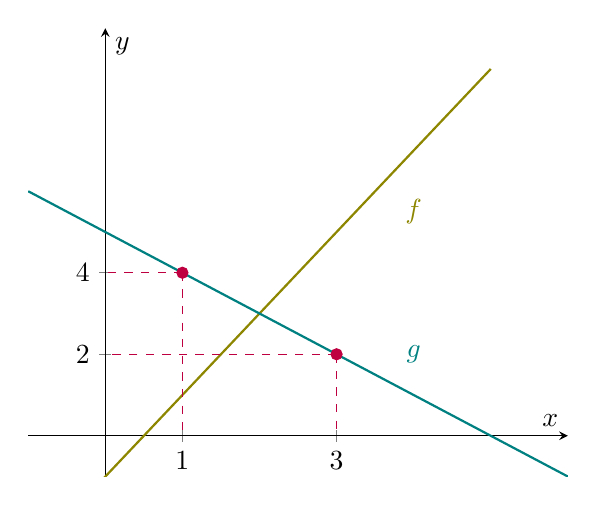
\begin{tikzpicture}
			\begin{axis}[
				axis lines = center, 
				xmin = -1, xmax = 6,
				ymin = -1, ymax = 10,
				xlabel = $x$, ylabel = $y$,
				xtick = {1,3}, ytick = {2,4}
				]
				\addplot[thick, color = olive] {2*x -1};
				\addplot[thick, color = teal, domain = -1:6] {-x + 5};
				\node[color = olive] at (axis cs: 4,5.5) {$f$};
				\node[color = teal] at (axis cs: 4,2) {$g$};
				\filldraw[color = purple] (axis cs: 1,4) circle (2pt);
				\filldraw[color = purple] (axis cs: 3,2) circle (2pt);
				\draw[color = purple, dashed] (axis cs: 1,4) -- (axis cs:1,0);
				\draw[color = purple, dashed] (axis cs: 1,4) -- (axis cs:0,4);
				\draw[color = purple, dashed] (axis cs: 3,2) -- (axis cs:3,0);
				\draw[color = purple, dashed] (axis cs: 3,2) -- (axis cs:0,2);
			\end{axis}
		\end{tikzpicture}
		\caption{Graferne for funktionerne $f$ og $g$.}
		\label{fig:linjer}
	\end{figure}
	Forskriften for $f$ er givet ved
	\begin{align*}
		f(x) = 2x -1.
	\end{align*}
\end{opgavetekst}
\begin{delopgave}{}{1}
	Bestem forskriften for $g$. 
\end{delopgave}
\begin{delopgave}{}{2}
	Bestem skæringspunktet mellem grafen for $f$ og grafen for $g$. 
\end{delopgave}
%%%%%%%%%%%%%%%%%%%%%%%%%%%%%%%%%%%%%%%%%%%%%%%%%%%%%%%%%%%%%%%%%%%%%%%%%%%%%%%%%%%%%%%%%%%%%%%%
%%%%%%%%%%%%%%%%%%%%%%%%%%%%%%%%%%%%%%%%%%%%%%%%%%%%%%%%%%%%%%%%%%%%%%%%%%%%%%%%%%%%%%%%%%%%%%%%
%%%%%%%%%%%%%%%%%%%%%%%%%%%%%%%%%%%%%%%%%%%%%%%%%%%%%%%%%%%%%%%%%%%%%%%%%%%%%%%%%%%%%%%%%%%%%%%%
%%%%%%%%%%%%%%%%%%%%%%%%%%%%%%%%%%%%%%%%%%%%%%%%%%%%%%%%%%%%%%%%%%%%%%%%%%%%%%%%%%%%%%%%%%%%%%%%
%%%%%%%%%%%%%%%%%%%%%%%%%%%%%%%%%%%%%%%%%%%%%%%%%%%%%%%%%%%%%%%%%%%%%%%%%%%%%%%%%%%%%%%%%%%%%%%%
%%%%%%%%%%%%%%%%%%%%%%%%%%%%%%%%%%%%%%%%%%%%%%%%%%%%%%%%%%%%%%%%%%%%%%%%%%%%%%%%%%%%%%%%%%%%%%%%
%%%%%%%%%%%%%%%%%%%%%%%%%%%%%%%%%%%%%%%%%%%%%%%%%%%%%%%%%%%%%%%%%%%%%%%%%%%%%%%%%%%%%%%%%%%%%%%%
%%%%%%%%%%%%%%%%%%%%%%%%%%%%%%%%%%%%%%%%%%%%%%%%%%%%%%%%%%%%%%%%%%%%%%%%%%%%%%%%%%%%%%%%%%%%%%%%
\newpage

\begin{center}
	\LARGE Med hjælpemidler
\end{center}


\begin{opgavetekst}{Opgave 6}
	\begin{center}
		
\includegraphics[width = 0.6\textwidth]{Billeder/helpizza}
	\end{center}	
	En pige har målt på diameteren og vægten af en række pizzaer. Resultatet af hendes målinger fremgår af \href{https://github.com/ChristianJLex/TeachingNotes/raw/master/2023-2024/Data og lign/Pizzavaegt.xlsx}{\color{blue!60} dette datasæt.} Hun har en antagelse om, at vægten af pizzaerne kan beskrives ved en sammenhæng af typen
	\begin{align*}
		M(x) = b \cdot x^a,
	\end{align*}
	hvor $M$ er vægten af pizzaen i gram og $x$ er diameteren af pizzaen i cm.
\end{opgavetekst}
\begin{delopgave}{}{1}
	Brug datasættet til at bestemme tallene $b$ og $a$.
\end{delopgave}	
\begin{delopgave}{}{2}
	Brug modellen til at bestemme vægten af en pizza med den diameter på 33 cm.
\end{delopgave}
%%%%%%%%%%%%%%%%%%%%%%%%%%%%%%%%%%%%%%%%%%%%%%%%%%%%%%%%%%%%%%%%%%%%%%%%%%%%%%%%%%%%%%%%%%%%%%%%
%%%%%%%%%%%%%%%%%%%%%%%%%%%%%%%%%%%%%%%%%%%%%%%%%%%%%%%%%%%%%%%%%%%%%%%%%%%%%%%%%%%%%%%%%%%%%%%%
%%%%%%%%%%%%%%%%%%%%%%%%%%%%%%%%%%%%%%%%%%%%%%%%%%%%%%%%%%%%%%%%%%%%%%%%%%%%%%%%%%%%%%%%%%%%%%%%
%%%%%%%%%%%%%%%%%%%%%%%%%%%%%%%%%%%%%%%%%%%%%%%%%%%%%%%%%%%%%%%%%%%%%%%%%%%%%%%%%%%%%%%%%%%%%%%%
%%%%%%%%%%%%%%%%%%%%%%%%%%%%%%%%%%%%%%%%%%%%%%%%%%%%%%%%%%%%%%%%%%%%%%%%%%%%%%%%%%%%%%%%%%%%%%%%
%%%%%%%%%%%%%%%%%%%%%%%%%%%%%%%%%%%%%%%%%%%%%%%%%%%%%%%%%%%%%%%%%%%%%%%%%%%%%%%%%%%%%%%%%%%%%%%%
%%%%%%%%%%%%%%%%%%%%%%%%%%%%%%%%%%%%%%%%%%%%%%%%%%%%%%%%%%%%%%%%%%%%%%%%%%%%%%%%%%%%%%%%%%%%%%%%
%%%%%%%%%%%%%%%%%%%%%%%%%%%%%%%%%%%%%%%%%%%%%%%%%%%%%%%%%%%%%%%%%%%%%%%%%%%%%%%%%%%%%%%%%%%%%%%%
\begin{opgavetekst}{Opgave 7}
	En potensfunktion $g$ er givet ved
	\begin{align*}
		g(x) = b \cdot x^4	
	\end{align*}
\end{opgavetekst}
\begin{delopgave}{}{1}
	Udnyt, at $g(2) = 13$ for at bestemme tallet $b$.
\end{delopgave}
\begin{delopgave}{}{2}
	Hvis vi ganger vores $x$-værdi med $2$, hvor meget øges funktionsværdien $g$ så med?
\end{delopgave}
%%%%%%%%%%%%%%%%%%%%%%%%%%%%%%%%%%%%%%%%%%%%%%%%%%%%%%%%%%%%%%%%%%%%%%%%%%%%%%%%%%%%%%%%%%%%%%%%
%%%%%%%%%%%%%%%%%%%%%%%%%%%%%%%%%%%%%%%%%%%%%%%%%%%%%%%%%%%%%%%%%%%%%%%%%%%%%%%%%%%%%%%%%%%%%%%%
%%%%%%%%%%%%%%%%%%%%%%%%%%%%%%%%%%%%%%%%%%%%%%%%%%%%%%%%%%%%%%%%%%%%%%%%%%%%%%%%%%%%%%%%%%%%%%%%
%%%%%%%%%%%%%%%%%%%%%%%%%%%%%%%%%%%%%%%%%%%%%%%%%%%%%%%%%%%%%%%%%%%%%%%%%%%%%%%%%%%%%%%%%%%%%%%%
%%%%%%%%%%%%%%%%%%%%%%%%%%%%%%%%%%%%%%%%%%%%%%%%%%%%%%%%%%%%%%%%%%%%%%%%%%%%%%%%%%%%%%%%%%%%%%%%
%%%%%%%%%%%%%%%%%%%%%%%%%%%%%%%%%%%%%%%%%%%%%%%%%%%%%%%%%%%%%%%%%%%%%%%%%%%%%%%%%%%%%%%%%%%%%%%%
%%%%%%%%%%%%%%%%%%%%%%%%%%%%%%%%%%%%%%%%%%%%%%%%%%%%%%%%%%%%%%%%%%%%%%%%%%%%%%%%%%%%%%%%%%%%%%%%
%%%%%%%%%%%%%%%%%%%%%%%%%%%%%%%%%%%%%%%%%%%%%%%%%%%%%%%%%%%%%%%%%%%%%%%%%%%%%%%%%%%%%%%%%%%%%%%%
\newpage
\begin{opgavetekst}{Opgave 8}
	En eksponentialfunktion $h$ er givet ved
	\begin{align*}
		h(x) = 12\cdot a^x
	\end{align*}
\end{opgavetekst}
\begin{delopgave}{}{1}
	Udnyt, at $h(2) = 11.3$ for at bestemme $a$.
\end{delopgave}
\begin{delopgave}{}{2}
	Bestem halverings/fordoblingskonstanten for $h$ alt efter om $h$ er voksende eller aftagende. 
\end{delopgave}